% TO DO: Melhorar forma como os dados estao sendo plotados no espaço
% definir metricas a serem apresentadas para validacao (media?)
% definir modelo final (depois de arrumar over fitting) e fazer TESTE
\documentclass[conference]{IEEEtran}
\IEEEoverridecommandlockouts

\usepackage{cite}
\usepackage[portuguese,brazil,english]{babel}
\usepackage{amsmath, amssymb, amsfonts}
\usepackage[utf8]{inputenc}
\usepackage{algorithmic}
\usepackage{graphicx}
\usepackage{textcomp}
\usepackage{subfig}
\usepackage{diagbox}
\def\BibTeX{{\rm B\kern-.05em{\sc i\kern-.025em b}\kern-.08em
    T\kern-.1667em\lower.7ex\hbox{E}\kern-.125emX}}
\begin{document}

\title{Relatorio da Atividade \#1}

\author{\IEEEauthorblockN{Barbara Caroline Benato}
\IEEEauthorblockA{
RA 192865\\
barbarabenato@gmail.com}
\and
\IEEEauthorblockN{Breno Leite}
\IEEEauthorblockA{
RA 192863\\
brenolleite@gmail.com}}

\maketitle

\section{Introdução}

Este trabalho tem como intuito explorar técnicas de regressão linear, a fim de encontrar o melhor modelo possível para predizer o ano de uma das música utilizadas no  Million Song Dataset. Este dataset é composto de diversas características sobre as músicas, o dataset não possuí nenhum áudio, apenas as features extraídas das mesmas.

Neste trabalho será utilizado um número menor de \emph{features} do dataset, por motivos de simplicidade. As features que serão utilizadas são referentes ao timbre da música, ao todo elas são 90 \emph{features}. Onde 13 dessas representam a média do timbre, enquanto as outras 77 representam a covariância do timbre.

O objetivo deste trabalho é mostrar os experimentos que foram desenvolvidor, com intuito de encontrar o melhor modelo para predizer os anos das músicas. Durante o trabalho as métricas de \emph{Mean Average Error} (MAE) e  \emph{Mean Absolute Error} (MAE), o primeiro tem como intuito representar a função de custo da regressão linear. Já o segundo, tem como intuito encontrar uma média do erro em relação aos anos preditos.

O trabalho será dividido da seguinte forma, na seção \ref{sec:base} alguns dados interessantes sobre a base serão mostrados. Em seguida, a seção \ref{sec:ativ} descreve as atividades desenvolvidas. A seção \ref{sec:meto} explica as métricas e formas aplicadas para os experimentos, que são mostrados na seção \ref{sec:exp}. Por fim, a seção \ref{sec:conc} finaliza o trabalho discutindo os principais aprendizados e os objetivos que foram atingidos.

\section{Million Song Dataset} \label{sec:base}

[Descrever probabilidades e distribuição do dataset. (Se tivermos espaco)]

\section{Atividades} \label{sec:ativ}

Um processo gradual foi utilizado para verificar a qualidade e custo de cada modelo nos dados da base. Primeiramente o dataset foi dividido entre treino e validação, para tal tarefa, foi utilizado o método de cross-validação conhecido como $k$-Fold. Após a divisão um método de regressão linear baseada em descida de gradiente foi utilizado como \emph{baseline} para a continuidade do desenvolvimento.

Também foi desenvolvida uma solução como \emph{baseline} que utiliza-se do método da equação normal, essa foi criada com o intuito de comparar o comportamento entre as duas técnicas. Ambos foram implementadas utilizando funções do pacote \emph{scikit-learn}, e desenvolvidas em \emph{Python}. As funções \emph{SDGRegressor} e \emph{LinearRegression} são responsáveis pelas técnicas de descida de gradiente e equação normal respectivamente.

Diversas modificações foram feitas em cima desses modelos, dentre elas estão, normalização dos dados, regularização, redução de dimensionalidade, escolha do \emph{learning rate}, além de modelos mais complexos utilizando-se de funções polinomiais de segundo e terceiro grau. Os resultados dessas técnicas serão discutidos na seção \ref{sec:exp}, o intuito é mostrar as diferenças entre os modelos e as decisões neste trabalho tomadas.

\section{Metodologia} \label{sec:meto}

Como dito anteriormente a base \emph{Million Song Dataset} é utilizada para os testes neste trabalho, os testes foram todos feitos utilizando um $10$-fold para mais robustez do sistema, esse parâmetro foi escolhido por um processo de testes. Em todos os testes os dados foram normalizados, o que ajuda o modelo tanto quanto em melhores predições como em menores possibilidades de \emph{overfitting}.

Os testes foram feitos utilizando dos \emph{baselines} descritos, descida de gradiente e equação normal. Os melhores resultados destes métodos foram escolhidos para testes com modelos mais robustos, a forma de escolha desses métodos foram tanto em performance como em tempo de execução de cada técnica. Em alguns casos a diferença entre dois métodos era muito pequena, porém o custo computacional era muito diferente entre ambos, sendo assim foi escolhido os modelos que são mais rápidos por falta de tempo para testes mais robustos.

Os testes deste trabalho podem ser divididos da seguinte forma:

\begin{itemize}
	\item \textbf{Comparação entre equação normal e descida de gradiente: } Neste experimento ambos os modelos usam modelos lineares dos dados, assim como o mesmo processo de normalização. Este experimento tem como objetivo comparar os resultados obtidos por ambas as técnicas, e mostrar pontos positivos de cada uma. Outro fato importante é que nesses experimentos o \emph{learning rate} utilizado é constante e tem valor 0.01, outro experimento tratará da escolha do \emph{learning rate} mais adequado.
	\item \textbf{Analisar curva de aprendizado: } Neste experimento o intuito é analisar o nível do melhor modelo obtido pelo \emph{baseline} de descida de gradiente, ou seja, deseja-se verificar indícios de \emph{overfitting}, \emph{underfitting} entre outros problemas que podem aparecer.
	\item \textbf{Comparar diferentes \emph{learning rates}: } O objetivo deste experimento é utilizar do modelo de descida de gradiente que obteve melhor resultados nos experimentos anteriores e aplicar diversos \emph{learning rates} com intuito de identificar o valor que mais satisfaz o problema. Isso significa, escolher um \emph{learning rate} que não prejudique a performance do algoritmo, mas que também não prejudique o aprendizado do mesmo.
	\item \textbf{Verificar modelos mais complexos: } Este experimento tem como objetivo analisar como equações de segundo e terceiro grau influenciam na capacidade de predição dos dados, iremos utilizar neste os parâmetros que obtiveram melhor sucesso nos outros experimentos.
	\item \textbf{Teste final: } Este experimento tem como intuito verificar como o modelo convergiu nos dados de teste, este foi utilizado somente uma vez no desenvolvimento do trabalho para a execução final dos testes. Desta forma, todos os dados do teste são totalmente novos para os modelos.
\end{itemize}

Por motivos de alto custo computacional do computo da equação normal, parte dos experimentos é voltada somente para o método de descida de gradiente. O mesmo acontece com o valor total de iterações da descida, por motivos de custo computacional apenas 100 iterações foram utilizadas.


%base: subset of the Million Song Dataset (descrever)
%explicar cada um deles e parametros utilizados
%sklearn:
%- pre processing: scale, normalize, pca
%- metodos: LinearRegression e SGDRegressor

%- base: subset of the Million Song Dataset (descrever)
%- treino validação (validação cruzada) e teste
%- metricas
%- graficos: learning\_curve e plot


\section{Experimentos e Discussões} \label{sec:exp}

Esta seção tem como objetivo mostrar os resultados obtidos no desenvolvimento do trabalho, assim como explicar as decisões nele tomadas. Vários outros experimentos foram feitos, como redimensionabilidade de \emph{features} usando PCA, diversas combinações de \emph{features}, porém apenas os melhores resultados obtidos serão mostrados aqui. Nas próximas seções as seguintes abreviações são utilizadas:

\begin{itemize}
	\item \textbf{M} - Somente as \emph{features} referentes média do timbre;
	\item \textbf{C} - Somente as \emph{features} referentes a covariância do timbre;
	\item \textbf{M/C} - \emph{features} de covariância e média do timbre;
	\item \textbf{M/C*} - \emph{features} de covariância e média do timbre sendo normalizadas separadamente.
\end{itemize}

\subsection{Equação Normal vs Descida de Gradiente}

Nesta seção serão mostrados os resultados obtidos para os modelos mais simples que é composto de uma função linear dos dados de entrada, assim como valores fixos para os parâmetros como o \emph{learning rate}. Experimentos mais a frente vão tratar de formas melhores de escolher esses parâmetros, nesta seção a preocupação é escolher as melhores \emph{features} a serem usadas assim como um modelo que possa ser posteriormente melhorado.

Depois de um processo de testes envolvendo combinações das \emph{features}, pode-se perceber que havia uma diferença entre usar todas elas, ou somente a variância ou o média do timbre. Neste experimento essas três alternativas foram testadas, a Tabela \ref{tab:feat} mostra os resultados obtidos utilizando a métrica MAE e utilizando diferentes \emph{features}.

\begin{table}[!h]
	\centering
	
	\begin{tabular}{ccccc} \hline
		\backslashbox{\textbf{Modelos}}{\textbf{Features}}  & \textbf{M/C*} & \textbf{M/C} & \textbf{C} & \textbf{M} \\ \hline
		\textbf{Gradiente} & 7,71          & 7,60         & 7,49       & 7,87       \\
		\textbf{Eq Normal} & 6,81          & 7,31         & 7,45       & 7,80      
	\end{tabular}
	
	\caption{Resultados da métrica Mean Absolute Error usando diferentes features.}
	\label{tab:feat}
\end{table}


Pode-se perceber que o uso de normalizações separadas paras a média e a covariância teve um grande impacto no resultado da equação normal, porém esse impacto não foi tão grande na descida de gradiente. Para o gradiente, usar apenas a covariância foi o melhor resultado. Porém analisar os dados desta forma, não é uma forma eficaz de determinar quais modelos estão mais aptos a predizer os dados do mundo real.

Para isso devemos analisar outras informações sobre o aprendizado, como a curva de aprendizado que será discutida na próxima seção.

\subsection{Curva de aprendizado}

Para escolher um dos modelos é necessário não só analisar suas taxas de erro, mas sim a forma com que o aprendizado ocorreu. Esperamos que esse modelo saiba generalizar em outros dados que não foram previamente vistos, a curva de aprendizado pode ajudar a decidir qual modelo tende a ser melhor em uma nova base de dados. Levando isso em conta, a Figura \ref{fig:learningcurves} mostra a curva de aprendizado dos modelos propostos para a descida de gradiente.


\begin{figure}[!h]
	\centering
	\subfloat[Curva de aprendizado para média do timbre.]{
		{
			\setlength{\fboxsep}{1pt}
			\setlength{\fboxrule}{1pt}
			\fbox{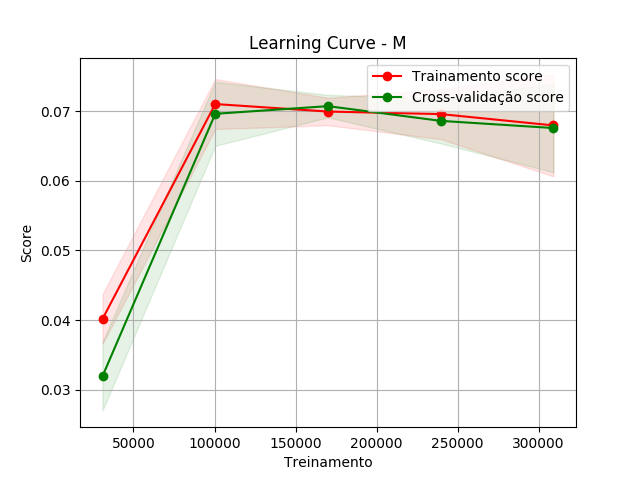
\includegraphics[scale=0.2]{../graphs/curveM.png}}
		}
	}
	\quad
	\subfloat[Curva de aprendizado para covariância do timbre.]{
		{
			\setlength{\fboxsep}{1pt}
			\setlength{\fboxrule}{1pt}
			\fbox{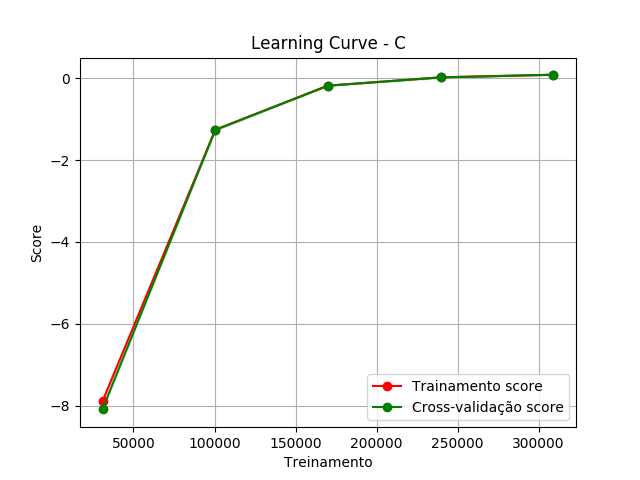
\includegraphics[scale=0.2]{../graphs/curveC.png}}
		}
	}
	\quad
	\subfloat[Curva de aprendizado para média e covariância do timbre.]{
		{
			\setlength{\fboxsep}{1pt}
			\setlength{\fboxrule}{1pt}
			\fbox{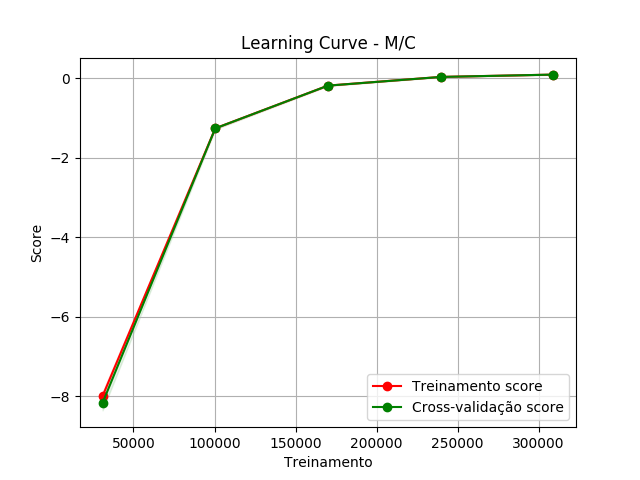
\includegraphics[scale=0.2]{../graphs/curveMC.png}}
		}
	}
	\quad
	\subfloat[Curva de aprendizado para média e covariância do timbre e normalização separada.]{
			{
				\setlength{\fboxsep}{1pt}
				\setlength{\fboxrule}{1pt}
				\fbox{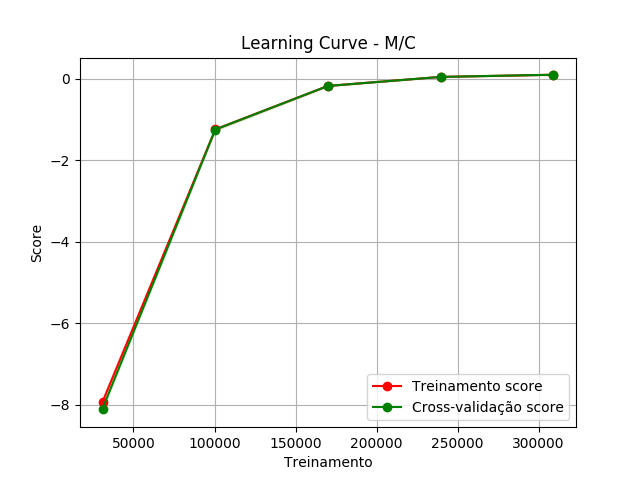
\includegraphics[scale=0.2]{../graphs/cuvreMC*.png}}
			}
		}
	\caption{Curvas de aprendizado para os diferentes modelos.}
	\label{fig:learningcurves}
\end{figure}

[Discutir sobre as imagens, acho que a C está melhor de todas, não tenho certeza pq ta negativo o score] [curveC trainamente sei que ta errado amanhã gero outro kkk]

\subsection{Learning Rate}

[Pensei em escolher uma das de cima e colocar 3 gráficos mais ou menos igual os do learning curve para 0.01, 0.001, e 0.0001]

\subsection{Modelos com equações de segundo e terceiro grau: }

\begin{table}[!h]
	\centering
	
	\begin{tabular}{ccccc} \\ \hline
		\backslashbox{\textbf{Modelos}}{\textbf{Features}} & \textbf{M/C*} & \textbf{M/C} & \textbf{C} & \textbf{M} \\ \hline
		\textbf{Gradiente}      & 7,54     & 7,63         & 7,50       & 7,63  \\  
		\textbf{Eq Normal}      & NA       & NA         & NA       & 7,58   
	\end{tabular}
	\caption{Resultados da métrica Mean Absolute Error usando diferentes features para as equações de segundo grau.}
	\label{tab:comp}
\end{table}

Nota-se que somente a média foi utilizado para a equação normal, o motivo deste é o alto custo do computo do mesmo para um grande número de \emph{features}. Poderia ter sido aplicado técnicas de redução de dimensionalidade, mas as mesmas já tinha se mostrado ineficazes para o problema. Desta forma, foi decidido não coletar essas informações.

Além disso, uma equação de terceiro grau foi utilizada para a descida de gradiente utilizando somente das \emph{features} de média do timbre. O resultado foi de 7,58 MAE, o que foi um pouco melhor que sua versão mais simples.

\subsection{Resultados na base de testes }

[Escolher alguns modelos e testar, ou testar todos os modelos (prefiro testar os 3 melhores, algo do tipo)]


%(Apresentar os dois graficos pra cada processo abaixo)\\

%>> LinearRegression\\
%--- Pre processamento\\
%- Modelo sem nenhuma alteraç~ao: resultado\\
%- Modelo com scale\\
%- Modelo com normalize\\
%- Modelo scale + normalize\\
%--- Feature Selection\\
%- Modelo com normalize + pca\\
%- Modelo buscando features: escolhe primeiras 10, primeiras 12, primeiras 13, primeiras 50, ultimas 78, ultimas 80\\
%---Definir modelo\\
%---Analisar overfitting do modelo\\
%--- validaç~ao cruzada: 3 / 5 / 10 folds\\
%- iteraç~oes: 50\\
%\\
%\\
%>> SGDRegressor \\
%--- Pre processamento\\
%- Modelo sem nenhuma alteração: resultado\\
%- Modelo com scale\\
%- Modelo com normalize\\
%- Modelo scale + normalize\\
%--- Feature Selection\\
%- Modelo com normalize + pca\\
%- Modelo buscando features: escolhe primeiras 10, primeiras 12, primeiras 13, primeiras 50, ultimas 78, ultimas 80\\
%--- Definir modelo\\
%--- Analisar overfitting do modelo\\
%--- validação cruzada: 3 / 5 / 10 folds\\
%- iterações: 50\\
%valores de alpha: 0.1/0.01/0.001/0.0001 + (?)\\

\section{Conclusão} \label{sec:conc}


\begin{thebibliography}{00}
\bibitem{b1} Christopher M. Bishop. ``Pattern Recognition and Machine Learning''. Springer-Verlag New York, Inc., Secaucus, NJ, USA, 2006.
\end{thebibliography}

\end{document}
